\documentclass[10pt,a4paper]{article}
\usepackage[margin=17mm]{geometry}
\usepackage[T1]{fontenc}
\usepackage{lmodern,amsmath,amssymb,graphicx,booktabs,array,xcolor,hyperref}
\hypersetup{colorlinks=true,urlcolor=blue,pdftitle={Actual rational Jacobian Richelot maps and the dual-only next hop}}
\setlength{\parindent}{0pt}\setlength{\parskip}{5pt}\setcounter{secnumdepth}{0}
\newcolumntype{L}[1]{>{\raggedright\arraybackslash}p{#1}}
\newcommand{\uv}{\texttt{[pcc:unverified]}}
\begin{document}
{\LARGE\bfseries Rational Jacobian Richelot maps}\par
{\large Full finite divisor-domain qualification and exact dual sign}\par
23 November 2026, 14:38 UTC \quad PR5007 \quad Source \texttt{4ae962c1}

\fcolorbox{blue!40!black}{blue!4}{\parbox{0.95\linewidth}{
\textbf{Observed result.} Four actual divisor-domain Richelot maps are
bijections on the $21$-class rational groups and pass $1{,}764$ map addition
checks. Both smooth codomains have only the dual rational kernel among all
$15$ matchings. All $84$ bidirectional composite classes equal the fixed
raw $-[2]$ expectation; all $80$ wrong-sign controls reject. Unsigned
data record \texttt{6b4fb5}; no signed PCC or Lean verdict. \uv}}

\begin{center}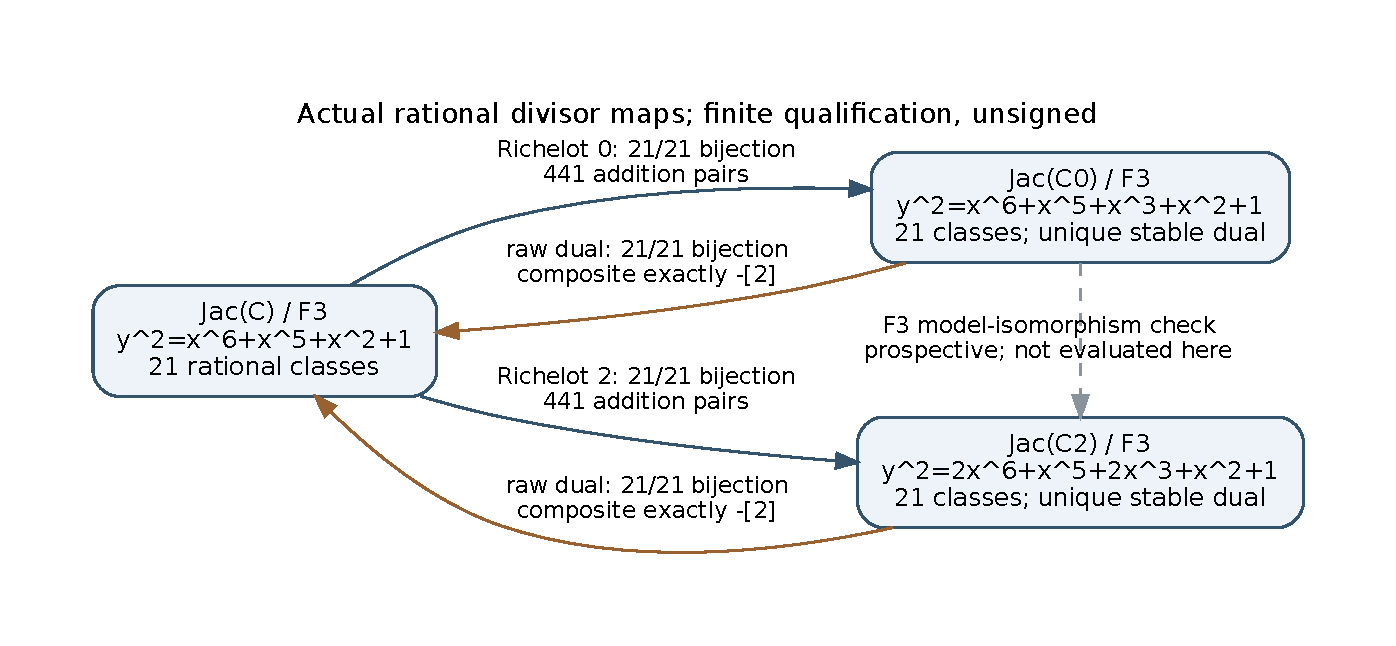
\includegraphics[width=0.98\linewidth]{maps.pdf}\end{center}
\vspace{-3mm}
\begin{center}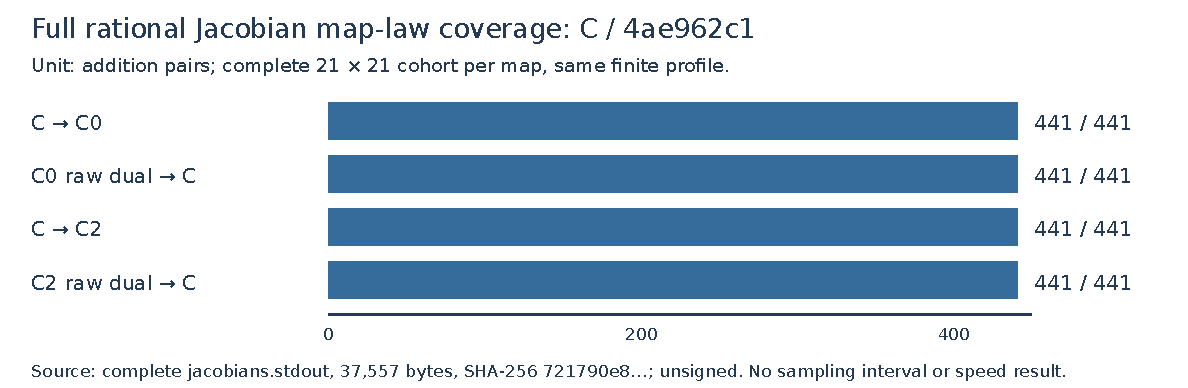
\includegraphics[width=0.92\linewidth]{coverage.pdf}\end{center}
\vspace{-3mm}

\section{Actual rational classes, not source scalar labels}
For each of the three exact displayed curves, enumerate all $12$ points
over $\mathbb F_9$ inside the qualified $\mathbb F_{729}$ tower. Exactly
$6$ are $\mathbb F_3$-rational. Frobenius-stable unordered degree-$2$ pairs,
including repetitions, give $24$ effective divisors and $21$ canonical
classes. Identity occurs four times; every other class occurs once.
Independent quadratic-support reconstruction recovers its actual point
pair. Full $441$ additions and $9{,}261$ addition-table associativity
triples pass for each group. Order counts are $1,2,6,12$ at orders
$1,3,7,21$. \uv

The map accepts only a divisor, source/target charts and a kernel.
Split its degree-$2$ Mumford support with multiplicity, evaluate ordinates,
recover homogeneous source points, apply the full Richelot point
correspondence and add the target divisors. For each of four maps,
all $24$ original effective-pair representatives independently agree,
$441$ scalar controls pass, and every output is valid and fixed by
corrected original $\mathbb F_3$ Frobenius. No scalar/class index enters
the transfer. \uv

\newpage
{\Large\bfseries Why the second rational kernel is the dual}\par

\section{Exact kernels and geometric sign}
The actual codomain branch permutations, in ascending root encoding, are
\[
 C_0:\ [5,4,3,1,0,2],\qquad C_2:\ [4,3,5,2,1,0].
\]
Both are six-cycles. A stable matching is a fixed-point-free involution
commuting with Frobenius. The centralizer of a six-cycle is its cyclic
group; the unique order-$2$ element is its cube. Thus the observed unique
stable matching has an elementary written explanation. This argument has
not been compiled in Mathlib. \uv

For factors $G_i$, brackets $H_i=G_jG_k'-G_j'G_k$ and determinant
$\Delta$, the fixed raw dual factors are
$(H_0/\Delta,H_1,H_2)$. Coefficient assertions check the bracket identities
and the raw second curve $4f=f$ in characteristic $3$.
The raw ordinate is $2y$; dividing it by $2$ identifies the usual dual.
Accordingly, both directions of both evaluated edges are exactly $-[2]$
on all $21$ classes. Restored negation equals $[2]$; the wrong $+[2]$
expectation disagrees on all $20$ nonidentity classes per direction and
agrees at identity. The sign was fixed before execution. \uv

\section{Controls, first failures and provenance}
\begin{center}\begin{tabular}{@{}L{0.31\linewidth}L{0.61\linewidth}@{}}
\toprule
Item & Complete retained outcome\\\midrule
Actual invalid inputs & Each curve's first tested constant-ordinate mutation
fails validity; real nonrational degree-$1$ classes fail rational eligibility.
A nonzero valid rational class is the positive counterpart.\\
Product endpoint & Actual original kernel with determinant $0$ is rejected.\\
First A & Versions $0$, formatting $1$; complete $21{,}277$ B diagnostic.\\
First B & Versions $0$, formatting $1$; complete $481$ B print-wrap diagnostic.\\
First C & All seven phases $0$; source/copy/tool/immutable-ELF guards unchanged.\\
Complete native raw & $37{,}557$ B stdout, SHA-256 prefix \texttt{721790e8};
all $63$ group classes, $84$ individual map outputs, $84$ composites,
all $30$ matchings and real controls.\\
Resource/custody & Rust1.99.1, shared Linux x86-64 development, $2$ GiB,
$120$ seconds per phase, one worker. Whole $4{,}784{,}904$ B ELFs,
SHA prefix \texttt{63e4738b}, remain RAM custody-pending.\\
\bottomrule\end{tabular}\end{center}

All $29$ frozen C inputs were completely read back from GitHub before
first phases. A/B sources and diagnostics are unchanged. C changes only
the observed B print-format hunk; no previous scientific population was
replayed. Full raw, phase and manifest records are in
\path{rational_jacobian/first-C-native/}; result JSON and
\path{rational_jacobian/CURRENT_RESULT_C.md} give exact bindings. \uv

\section{Scope and the next discriminating check}
The zero-nondual result concerns rational Richelot kernels on these two
exact codomains. It does not classify model isomorphisms, routes through
products, extension-field composites or other curves. Next explicitly
enumerate $\operatorname{PGL}_2(\mathbb F_3)$ changes between the three
models and evaluate any resulting cross-model chains. A source involution
may relate the two smooth kernels; the dashed diagram edge is prospective.
Cold comparative costs, actual Weil-$8$, generic Mathlib and normal
CI/custody gates remain open. No performance comparison was run. \uv

\begin{flushleft}\footnotesize
Sources: qualified native field/chart/Cantor bytes from \texttt{269689ea};
\path{RATIONAL_JACOBIAN_CHAIN_LEAD.md}; Magma Richelot handbook1615;
Bruin--Doerksen \href{https://arxiv.org/abs/0902.3480}{0902.3480v3}.
KB/Conductor unavailable, exact-source fallback, no novelty clearance.
Char-$3$ identities have native coefficient checks; the existing fixed
$2^{61}-1$ identity-certificate format and generic Lean bridges do not
certify them. \uv\quad
\href{https://github.com/isogeny-labs/crypto/pull/5007}{PR5007}\quad
\href{https://github.com/isogeny-labs/crypto/issues/3904}{Queue3904}
\end{flushleft}
\end{document}
